\documentclass{beamer}

\input{/home/tim/Documents/Ecole/modele_diapositives.tex}

\institute{INSA de Rouen Normandie}
\logo{
\includegraphics[width=70px]{img/logo.png}}

\lstset{
language=Matlab,
morekeywords={switch,case,otherwise},
tabsize=2
}

\usetheme{Warsaw}
\setbeamercovered{transparent}
\setbeamertemplate{itemize item}[triangle]
\expandafter\def\expandafter\insertshorttitle\expandafter{%
  \insertshorttitle\hfill%
  \insertframenumber\,/\,\inserttotalframenumber}

\begin{document}
\title{Soutenance mi-parcours PFE}  
\author{Timothée Schmoderer}
\date{\today} 

\begin{frame}[plain]
\titlepage
\end{frame}

\begin{frame}[plain]
\frametitle{Sommaire}
\tableofcontents
\end{frame}


\section{Introduction} 
\frame{\frametitle{Introduction} 
\begin{itemize}
\item Gaspard Monge 1871 - \emph{Mémoire sur la théorie des déblais et des remblais}
\item Leonid Kantorovitch 1942
\item JD. Benamou et Y. Brenier 2000
\end{itemize}
}
\subsection{Définitions}
\frame{ 
\begin{definition}{Transport}
Soient $2$ mesures de probabilités $\mu$ et $\nu$ sur $\mathcal{R}^N$. \\
Un transport est une application $T:\mathbb{R}^N\rightarrow\mathbb{R}^N$ qui envoie $\mu$ sur $\nu$, càd. : 
\begin{align}
\forall B\in \mathcal{B}\left(\mathbb{R}^N\right) \quad \mu\left(T^{-1}(B)\right) = \nu(B)
\label{eq:transport}
\end{align}
\end{definition}


C'est une relation de conservation de masse. On note $T_{\#}\mu =\nu$.
}
\frame{
\begin{block}{}
Supposons que $\mu =f_0dx$, $\nu = f_1dx$ et $T\in \mathcal{C}^1$ alors (\ref{eq:transport}) devient :
\begin{align}
\int_Bf_1(y)dy &=\int_{T^{-1}(B)}f_0(x)dx\\
&=\int_B \sum_{x\in T^{-1}(y)}\left( \frac{f_0(x)}{|\nabla T(x)|}\right) dy
\label{eq:regularTransport}
\end{align}
\end{block}
}

\frame{
\begin{block}{Définition : Problème de transport optimal}
Notons $\mathcal{T}(f_0,f_1)$ l'ensemble des applications transport qui vérifient (\ref{eq:regularTransport}). \\
On se donne un coût : $C:\mathbb{R}^N\times\mathbb{R}^N\rightarrow\mathbb{R}^+$.
Le problème de transport optimal est alors de trouver $T\in \mathcal{T}(f_0,f_1)$ qui réalise le 
$$
\min_{T\in\mathcal{T}(f_0,f_1)}  \int C\left(x,T(x)\right) dx
$$
Dans notre cas, $C(x,y) = \|x-y\|^2$. La valeur minimale est alors appelée distance $L^2$ de Wasserstein entre $f_0$ et $f_1$.
\end{block}
}

\section{Reformulation du problème} 

\frame{
\frametitle{Reformulation du problème}

\begin{theoreme}{Benamou et Brenier}
Soient deux densités de probabilités $f_0dx$ et $f_1dx$ alors 
\begin{align*}
\min_{T\in\mathcal{T}(f_0,f_1)}  \int \|x-T(x)\|^2 &dx = \\
& \min_{(\rho,v)\in C_v}\frac{1}{2}\int_{\mathbb{R}^N}\int_0^1 \rho(t,x)\|v(t,x)\|^2dtdx
\end{align*}
\end{theoreme}
 
\begin{itemize}
\item $\rho:\mathbb{R}\times\mathbb{R}^N\rightarrow\mathbb{R}$ est la densité $> 0$.
\item $v :\mathbb{R}\times\mathbb{R}^N\rightarrow\mathbb{R}^N$ est un champ de vitesses.
\item $C_v=\left\{(\rho,v)\ |\ \partial_t\rho +div_x(\rho v)=0,\ \rho(0,\dot)=f_0,\ \rho(1,\dot)=f_1\right\}$
\end{itemize}
}

\frame{
\begin{block}{}
On pose, $m = \rho v$ et :
$$
J(t,x) =
\left\{
\begin{array}{ccl}
\frac{\|m(t,x)\|^2}{\rho(t,x)}& \text{ si }& \rho(t,x) >0\\
0& \text{ si }& (\rho(t,x),m(t,x))= (0,0)\\
+\infty& \text{ sinon }\\
\end{array}
\right.
$$
De sorte que : 
$$
C_v=\left\{(\rho,mv)\ |\ \partial_t\rho +div_x(m)=0,\ \rho(0,\bullet)=f_0,\ \rho(1,\bullet)=f_1\right\}
$$
\end{block}

On remarque que, si $\rho\rightarrow +\infty$ alors $J(t,x)\rightarrow 0$ donc la fonctionnelle n'est pas coercive ce qui rend l'existence minimiseurs non trivial. Et si $\rho\rightarrow 0$ alors $J(t,x)\rightarrow +\infty$ donc le gradient n'est pas lipschitz, ce qui nous empêche d'utiliser les algorithmes de minimisation classique comme (algorithme du gradient conjugué). 
}


\section{Introduction aux opérateurs proximaux} 
\frame{
\frametitle{Introduction aux opérateurs proximaux}

}


\section{Attaque numérique du problème}
\frame{
Dans ce qui suit, on se place en dimension $1$ en espace. 
\begin{block}{Algorithme DR appliqué au problème de transport}
Le problème se reformule sous la forme : 
\begin{align*}
min_{w=(m,\rho)\in \mathcal{H}} J(w) + \mathbf{i}_C(w)
\end{align*}
Ainsi, étant donné $(z_0,w_0)\in\mathcal{H}^2$ 
$$
\left\{
\begin{array}{ccl}
w_{n+1} &=& w_n+\alpha\left(Prox_{\gamma J}(2z_n-w_n)-z_n\right)\\
z_{n+1} &=& Prox_{\gamma \mathbf{i}_C}(w_{n+1})
\end{array}
\right.
$$
\end{block}
}
\begin{frame}
\frametitle{Grille}
\begin{block}{Discrétisation}
On se donne deux entiers $N$ et $P$. On divise le carré espace temps $[0,1]^2$ en $(P+1)\times(N+1)$ points.\\
On note $\mathcal{G}_c$ cette grille est $w_{ij}$ la variable w discrétisée.


\attention{ $i$ parcours l'axe spatial (les colonnes donc) et $j$ l'axe temporel (les lignes).}
\end{block}
\end{frame}

\begin{frame}
\frametitle{Opérateur proximal de $\gamma J$}
\begin{block}{Proposition}
$$
\forall w  \quad Prox_{\gamma J} = (Prox_{\gamma J} (w_{ij})_{ij\in\mathcal{G}_c}
$$
Où, pour tout $w_{ij}=(m_{ij},f_{ij})$ on a : 
$$
Prox_{\gamma J} = \left\{
\begin{array}{ccl}
(\frac{f_{ij}^{\star}m_{ij}}{f_{ij}^{\star} + \gamma},f_{ij}^{\star}) & si\ f_{ij}^{\star} >0\\
(0,0) & sinon
\end{array}\right.
$$

Et, $f_{ij}^{\star}$ est la plus grande solution réelle du polynôme de degré 3 : 
$$
P(x) = (X - f_{ij})(X+\gamma)^2 - \frac{\gamma}{2}\|m_{ij}\|^2
$$

\end{block}
\end{frame}

\begin{frame}
\frametitle{Opérateur proximal de $\mathbf{i}_C$}
L'opérateur proximal de $\mathbf{i}_C$ est l'opérateur de projection sur l'ensemble convexe $C$. On reformule cette ensemble sous forme affine : 
$$
C = \left\{w\ |\ Aw = y \right\}
$$
Où, 
$$
Aw = (div(m) +\partial_t \rho,\ \rho (\bullet,0),\ \rho (\bullet ,1)) \quad y = (0,f_0,f_1)
$$
Finalement, on obtient : 
$$
Proj_C(\bullet) = (Id-A^{\star}\Delta^{-1}A)\bullet + A^{\star}\Delta^{-1}y \qquad \Delta^{-1} = (AA^{\star})^{-1}
$$
\end{frame}


\subsection{La plus simple}
\frame{
\begin{block}{Principe}
Représentation des données sur la grille centrée. 
Méthode de gradient conjugué pour évaluer $Proj_C$.
\end{block}
\begin{exampleblock}{Avantages}
	\begin{itemize}
	\item rapidité de mise en oeuvre 
	\item extensible facielement en dimension N 
	\end{itemize}
\end{exampleblock}
\begin{alertblock}{Inconvénients}
	\begin{itemize}
	\item asymétrie de la dérivée
	\end{itemize}
\end{alertblock}
}

%\subsection{la plus brutale}
%\frame{
%\begin{exampleblock}{Avantages}
%	\begin{itemize}
%	\item rapidité de mise en oeuvre 
%	\item calcul rapide
%	\end{itemize}
%\end{exampleblock}
%\begin{alertblock}{Inconvénients}
%	\begin{itemize}
%	\item matrices très mal conditionnées
%	\item extension en dimension supérieur impossible
%	\end{itemize}
%\end{alertblock}
%}
\subsection{la plus dure}
\frame{
\begin{block}{Principe}
Introduire des grilles décalées pour gérer le terme de divergence plus efficacement. Et rajouter une contrainte liant les variables décalées et les variables centrées. 
\end{block}

\begin{exampleblock}{Avantages}
	\begin{itemize}
	\item Précision
	\end{itemize}
\end{exampleblock}
\begin{alertblock}{Inconvénients}
	\begin{itemize}
	\item Difficile à mettre en œuvre
	\end{itemize}
\end{alertblock}
}

\section{Exemples}
\subsection{Exemple 1}
\frame{
\frametitle{Exemple 1}
\begin{figure}[!h]
\centering
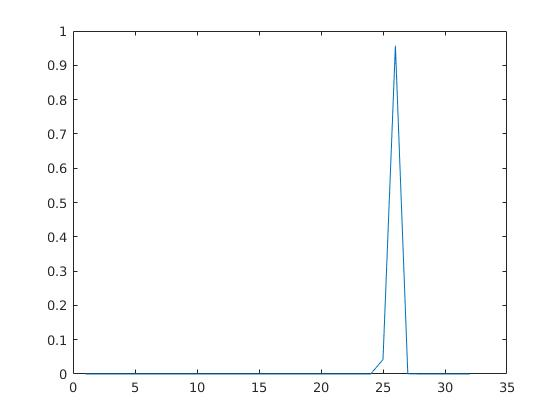
\includegraphics[height=120px]{../../results/gauss_f0.jpg}
\caption{$f_0$}
\end{figure}
}

\frame{
\frametitle{Exemple 1}
\begin{figure}[!h]
\centering
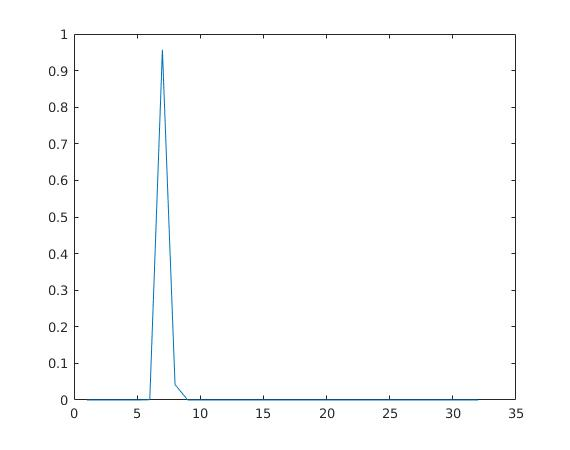
\includegraphics[height=120px]{../../results/gauss_f1.jpg}
\caption{$f_1$}
\end{figure}
}

\frame{
\frametitle{Exemple 1}
\begin{figure}[!h]
\centering
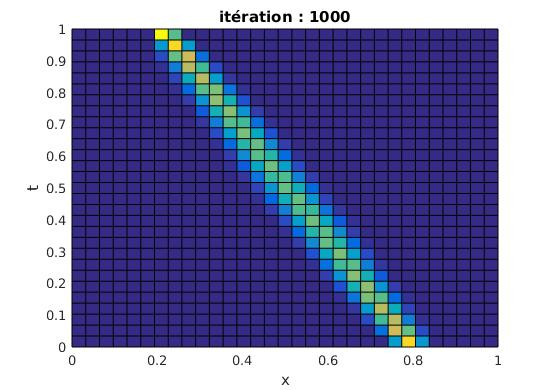
\includegraphics[height=120px]{../../results/gauss_transport.jpg}
\caption{Transport $f_0$ sur $f_1$}
\end{figure}
}

\subsection{Exemple 2}
\frame{
\frametitle{Exemple 2}
\begin{figure}[!h]
\centering
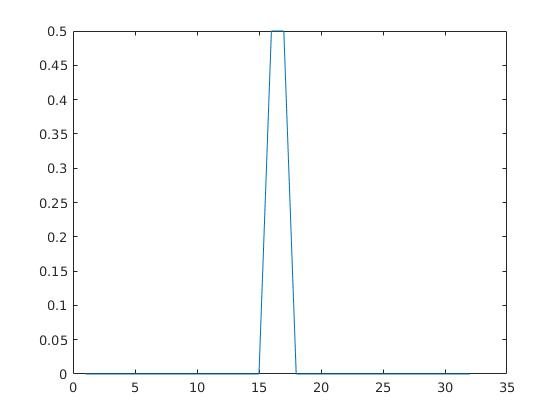
\includegraphics[height=120px]{../../results/gauss_mixture_f0.jpg}
\caption{$f_0$}
\end{figure}
}

\frame{
\frametitle{Exemple 2}
\begin{figure}[!h]
\centering
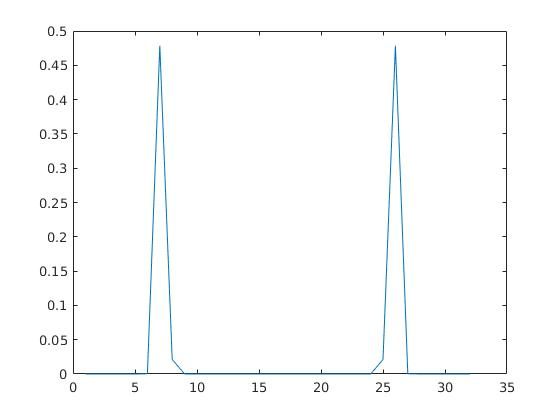
\includegraphics[height=120px]{../../results/gauss_mixture_f1.jpg}
\caption{$f_1$}
\end{figure}
}

\frame{
\frametitle{Exemple 2}
\begin{figure}[!h]
\centering
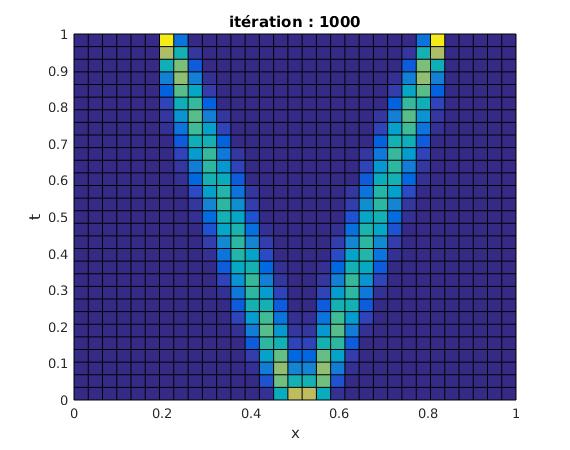
\includegraphics[height=120px]{../../results/gauss_mixture_transport.jpg}
\caption{Transport $f_0$ sur $f_1$}
\end{figure}
}

\subsection{Exemple 3}
\frame{
\frametitle{Exemple 3}
\begin{figure}[!h]
\centering
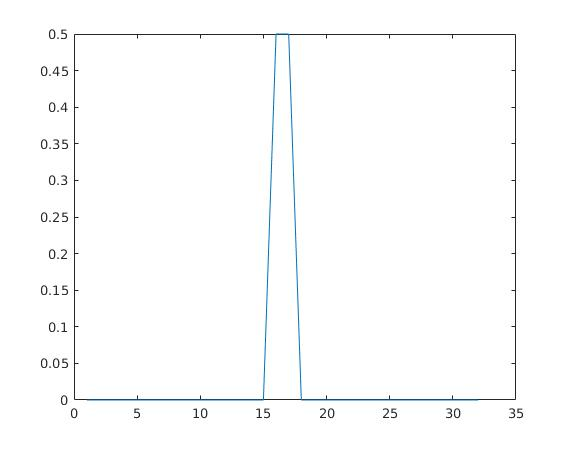
\includegraphics[height=120px]{../../results/gauss_sharp_f0.jpg}
\caption{$f_0$}
\end{figure}
}

\frame{
\frametitle{Exemple 3}
\begin{figure}[!h]
\centering
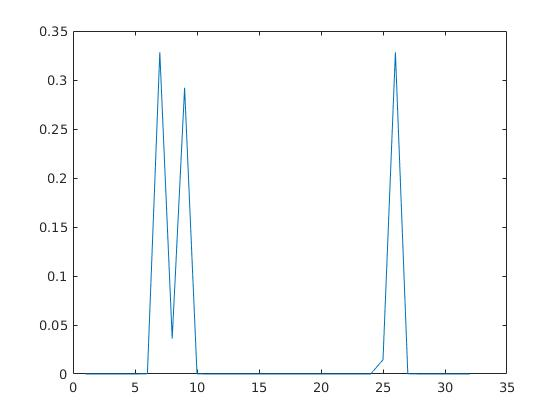
\includegraphics[height=120px]{../../results/gauss_sharp_f1.jpg}
\caption{$f_1$}
\end{figure}
}

\frame{
\frametitle{Exemple 3}
\begin{figure}[!h]
\centering
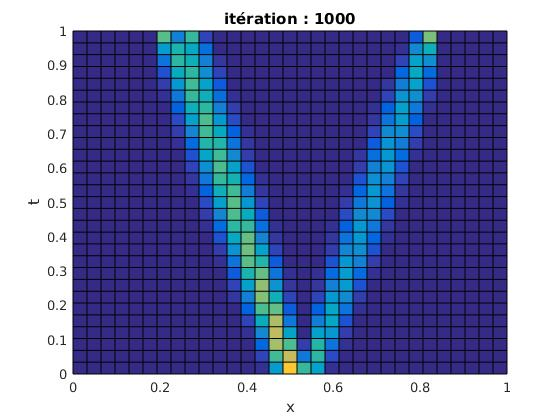
\includegraphics[height=120px]{../../results/gauss_sharp_transport.jpg}
\caption{Transport $f_0$ sur $f_1$}
\end{figure}
}




\end{document}

